\mychapter{2}{Randomness and Obfuscation}
\begin{center}
	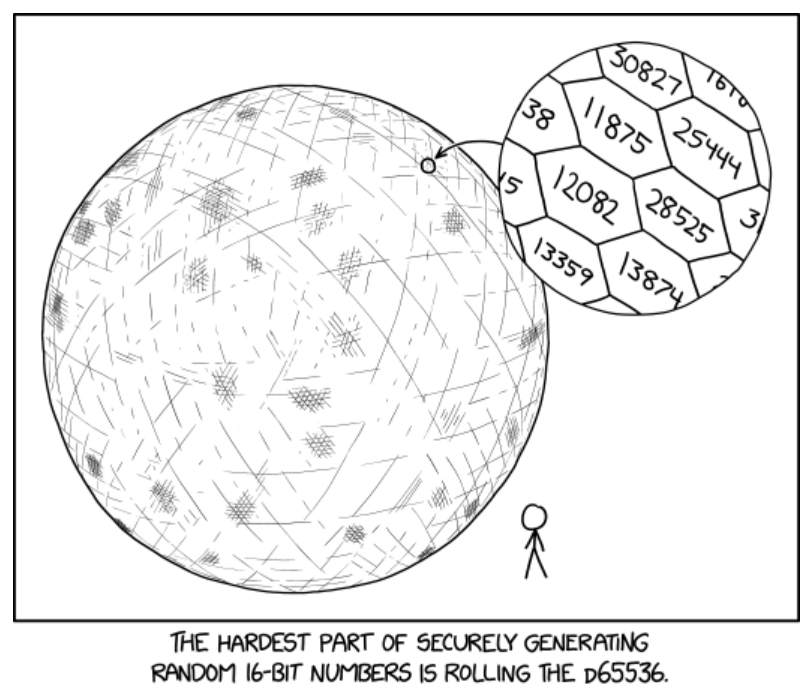
\includegraphics[width=0.75\textwidth]{Photos/random.png}
\end{center}
	\mysection{1}{Random Numbers}
		\subsection{Why do we need random numbers}
			A lot of the encryption techniques used in the later weeks will require some randomness to increase the strength of the cipher. We had already covered their importance in general in \textcolor{teal}{\hyperref[subsec:random]{Random Bit Sequences}} but in specific-
			\begin{itemize}
				\item RSA cryptosystems, despite being completely deterministic, requires some randomness in the plaintext for better security.
				\item Public key cryptosystems depend almost completely on the using random prime numbers to design the keys.
				\item Probabilistic Encryption systems definitely require incorporation of randomness into the encryption process.
			\end{itemize}

		\subsection{Is it even possible to construct an actually random number?}
			Quantum Theory states that the decay of specific atom is completely probabilistic. We can be sure that for a radioactive atom, there is a T time such that after T seconds, a undecayed atom has a \emph{50\%} chance of decaying but we cannot say with 100\% surety if a particular atom will decay or not.\par
			Thus to construct the first bit of a random number, we just study a radioactive atom for T seconds and if it decays, $bit = 1$ else $bit = 0$. \par
			Unfortunately, this is a very impractical way to construct a large random string daily use. Hence we go for pseudo random bit generators.

		\subsection{Pseudo-Random Number Generator}\label{subsec:prng}
			PRNG is just a function that takes in an initial seed \emph{S} which is truly random to algorithmically create a pseudo-random number\footnote{Called so because of the irony of having a well defined function that can create supposedly random numbers.}.\par
			The two properties that a PRNG should have for it to be considered cryptographically secure are-
			\begin{enumerate}
				\item If \emph{Eve} has the first \emph{k} bits of the PRN, she should not be able to predict the next bit with a more than 50\% chance.
				\item If \emph{Eve} has some the bits in the PRN such as \(R_t, R_{t+1}, R_{t+2} \cdots\), she should not be able to predict any of \(R_1, R_2, \cdots , R_{T-1}\) bits with a more than 50\% surety.
			\end{enumerate}

			To continue further, some knowledge of Hash Functions is necessary.

\begin{mdframed}
	\mysection{2}{Hash Functions}
		\centering \emph{Hash Algorithmns are like a summary of the original document. It is difficult to figure out the original document from the hash output but it acts as a signature that ensures accuracy. Due to the pigeonhole problem, it is obvious that Hash collisions would occur- but a good algorithm ensures that those are incredibly difficult to happen by happenstance and equally so to artificially bring about \\ \raggedleft{- Tom Scott}}\par
		
		\raggedright Hash functions take in arbitrarily long documents \(D\) and output a shorter bit strong \(H\). Their main objective is for authentication purposes. Some important characteristics are-
		\begin{itemize}
			\item Computation of $Hash(D)$ should be fast \(\rightarrow\) \emph{linear time}
			\item Inversion of Hash(D) should be difficult \(\rightarrow \) \emph{exponential time} i.e. finding \textbf{any} \emph{D} given a hash output \(H\) of the form \(Hash(D) = H\)
			\item Ideally we want Hash functions to have collision resistance i.e. it should be difficult for 2 non-identical documents \(D1\) and \(D2\) to give the \(Hash(D1)= Hash(D2)\). This property is important for the sake of unambiguity in differentiating between 2 possible inputs when the inteded recepient receives the Hash output.
		\end{itemize}
		\textbf{Note-} \\
		\quad a. There is a considerable difference between Authentication/ Verification and Inversion. Hash functions need to be easy to compute as well as verify but should be resistant from inversion. \\
		\quad b. Hash is not an encryption- it cannot (ideally) be decrypted back to the original message. It is just a signature.\\
		\quad c. Hash outputs are ``seemingly'' random so even a small flipping of bits in the input should completely change the hash. \par

		We ideally would base Hash functions on mathematically difficult problems to solve such as the Discrete Logaritms and Prime Factoring to ensure that inversion is difficult but that is impractical for even the encryption speeds today's world needs. So we prefer ad-hoc mixing methods such as the \emph{Secure Hash Algorithm} {SHA (or SHA-1)}  which is the universally used algorithm. 
		\subsection{How does SHA-1 work?}
		SHA outputs 160 bits no matter what you input in; if the input is a multiple of 160 bits, we just xor the first result of the \(k\)th output with the transformation of the (\(k+1\))th mixing to get the \(k+1\)th output. If the file isn't a multiple or is smaller than 160 bits, we just append 0s till we get a proper multiple. 
			\begin{enumerate}
				\item Choose 5 32-bit numbers \(h_0, h_1, h_2, \ldots, h_4\) randomly.
				\item Divide the file into chunks of 512 bits and then redivide those chunks individually into 16 blocks of 32-bits (or words) \(w_0, w_1, w_2\ldots w_15\).
				\item ``Rotate'' the words (i.e. shift the bits circularly arbitrarily \textbf{between} the words\footnote{Essentially if you have 1000, 1101, 0111, 1010 and you decided to rotate the 3rd bit in each 4-bit number, you can get a 1000, 1111, 0111, 1000 i.e. the 3rd bit of each number is extracted to form the array {0,0,1,1} and this is rotated as the algorithm is designed} (not inside the words individually)) to create 80 words \(w_0, w_1, w_2, \ldots, w_{79}\).
				\item Start the loop with i as control variable incrementing from 0 to 79. 
				\item Now just create temporarily variables \(a=h_0\), \(b=h_1, \; \ldots e=h_4\) and construct \(f\) from some arbitrary combination of \(a, b, c, d, e\) using AND and XOR.
				\item Arbitrarily mix \(a, b, c, d, e\) using some rotations, shifts and whatever you feel like adding on a lazy Wednesday afternoon.
				\item Add f and \(w_i\) to a and then equate \(h_0=h_0+a, h_1=h_1+b, \ldots ,h_4=h_4+e\).
				\item End the loop once you reach i=79. (i.e. complete 80 rounds)
				\item Do the same for all chunks just making sure that the values of \(h_0, h_1\ldots h_4\) are carried forward after each chunk.
				\item Concatenate \(h_0, h_1\ldots h_4\) to get the final 160-bit hash.
			\end{enumerate}
\end{mdframed}
			
			Thus now to create a pseudo-random number \(R_i\), we just select a specific \(Hash\) function and input into it \(S\) (A truly random number) concatenated with \(i\) to get-\[Hash(i\;||\;S)=R_i\] 

	\mysection{3}{Public Standard for making PRNGs}
		Start of with a random seed \(S\) and a key \(k\) for the cryptosystem. Let \(E_k\) be the encryption function associated with that \(k\). \\
		Every time a random number is required, create a \(D\) from some CPU parameters (temperauture and/or date and time and/or cpu usage) to get- \[C=E_k(D)\]
		Thus your random number \(R\) will be- \[R=E_k(C\; \text{xor}\; S)\]
		You can then update \(S\) to - \[S=E_k(R \;\text{xor}\; C)\]

	\mysection{4}{Stream Ciphers}
		\emph{This is an encryption technique which heavily depends on the PRNGs we defined above.}\\
		If you wanted to encrypt a 10-bit plaintext using Stream Ciphers, you will require a 10-bit keystream as well. If \(k_i\) is the \(i\)th bit of the keystream and \(m_i\) is the \(i\)th bit of the plaintext, \[c_i \equiv k_i \oplus m_i\] This keystream should be as random as possible to prevent codebreakers from predicting properties about the keystream thus getting information about the plaintext. \par
		But it is infeasible to make \(n\)-bit keystreams for large values of \(n\) hence we use PRNGs. We can thus have a \(k\) bit purely random seed \(S\) with which we can create \(R_1, R_2, R_3 \ldots, R_n\) using the above given algorithm. (Initial seed \(S\) is updated after every use as was defined in the last section to strengthen the security of the system)\par
		
		\begin{tcolorbox}\label{box:onetimepad}
			\textbf{BTW} the keystream used with Stream Ciphers is known as \emph{One Time Pad}. A \emph{n}-bit ciphertext made from a truly random \emph{n}-bit one time pad is mathematically impossible to decipher.
		\end{tcolorbox}
		
		\subsection{Deciphering Stream Ciphers}
			xor ($\oplus$) has an interesting property \(\rightarrow\)
			\begin{center}
			\begin{tabular}{ c | c | c | c}
				 $A$ & $B$ & $A \oplus B$ & $(A \oplus B) \oplus B$\\ 
				 \hline
				 0 & 0 & 0 & 0\\  
				 0 & 1 & 1 & 0\\
				 1 & 0 & 1 & 1\\
				 1 & 1 & 0 & 1   
			\end{tabular}
			\end{center}
			Hence we can say with surety that-
			\[k_i \oplus c_i \equiv k_i \oplus (k_i \oplus m_i) \equiv m_i\]
			Giving us a clear cut way to use this private key symmetric encryption system.\par
			\textbf{ALSO} since the generation of \(R_n\) does not require any subsequent \(R_{k>n}\), we can process each bit as it the CPU reads it instead of having to store it
	\mysection{5}{Block Cipher}
		Unlike Stream Cipher, Block Cipher is a lot simpler and less secure. It divides the input into chunks of bits and evaluates them separately.\footnote{A lot of these concepts and pictures are sourced from ``https://www.hypr.com/black-cipher/''} 

		\subsection{Electronic Code Book Method}
			Essentially if you have a \(k\) bit codebook and a \(n\) bit plain text, you divide the plain text into chunks of \(k\) bits (some padding scheme is employed in case \(n\;\% \;k \not = 0\)). Then you go through each chunk and find the corresponding ciphertext in the ECB (Electronic Code Book). Thus you encrypt the entire file.
			\begin{center}
			\begin{tabular}{ c | c }
				 $Plaintext$ & $Ciphertext$ \\ 
				 \hline
				 00 & 11\\   
				 01 & 01\\
				 10 & 00\\
				 11 & 10    
			\end{tabular}
			\end{center}
			\centering\emph{{2-bit Electronic Code Book}}

			\begin{mybox}
				\raggedright \LARGE{\textbf{Some minor itty bitty issues}}- \normalsize It preserves large scale structures hence it is completely useless to the most degree in obfuscating files with a large size if there is a lot of repetition.
			\end{mybox}

			Imagine a $10\times10$ picture where the brightness of each pixel is defined by a 2-bit digit
			\begin{center}
			\begin{tabular}{ c | c }
				 $Plaintext$ & $Ciphertext$ \\ 
				 \hline
				 0000 & 1001\\  
				 0001 & 1000\\
				 0010 & 0100\\
				 0011 & 0101\\
				 0100 & 0011\\
				 0101 & 0111\\
				 0110 & 1101\\
				 0111 & 1111\\
				 1000 & 0110\\  
				 1001 & 1011\\
				 1010 & 0001\\
				 1011 & 1100\\
				 1100 & 0010\\
				 1101 & 1100\\
				 1110 & 1010\\
				 1111 & 0000
			\end{tabular}
			\end{center}
			\centering\emph{{4-bit Electronic Code Book}}

			\[
				\begin{bmatrix}
					\color{red}00 & \color{red}00 & \color{red}00 & \color{red}00 & \color{red}00 & \color{red}00 & \color{red}00 & \color{red}00 & \color{red}00 & \color{red}00\\
					\color{red}00 & \color{red}00 & \color{red}00 & \color{red}00 & \color{red}00 & \color{red}00 & \color{red}00 & \color{red}00 & \color{red}00 & \color{red}00\\
					\color{red}00 & \color{red}00 & \color{blue}01 & \color{blue}01 & \color{blue}01 & \color{blue}01 & \color{blue}01 & \color{blue}01 & \color{red}00 & \color{red}00\\
					\color{red}00 & \color{red}00 & \color{blue}01 & \color{yellow}\color{yellow}10 & \color{yellow}10 & \color{yellow}10 & \color{yellow}\color{yellow}10 & \color{blue}01 & \color{red}00 & \color{red}00\\
					\color{red}00 & \color{red}00 & \color{blue}01 & \color{yellow}10 & \color{green}11 & \color{green}11 & \color{yellow}10 & \color{blue}01 & \color{red}00 & \color{red}00\\
					\color{red}00 & \color{red}00 & \color{blue}01 & \color{yellow}10 & \color{green}11 & \color{green}11 & \color{yellow}10 & \color{blue}01 & \color{red}00 & \color{red}00\\
					\color{red}00 & \color{red}00 & \color{blue}01 & \color{yellow}\color{yellow}10 & \color{yellow}10 & \color{yellow}10 & \color{yellow}\color{yellow}10 & \color{blue}01 & \color{red}00 & \color{red}00\\
					\color{red}00 & \color{red}00 & \color{blue}01 & \color{blue}01 & \color{blue}01 & \color{blue}01 & \color{blue}01 & \color{blue}01 & \color{red}00 & \color{red}00\\
					\color{red}00 & \color{red}00 & \color{red}00 & \color{red}00 & \color{red}00 & \color{red}00 & \color{red}00 & \color{red}00 & \color{red}00 & \color{red}00\\
					\color{red}00 & \color{red}00 & \color{red}00 & \color{red}00 & \color{red}00 & \color{red}00 & \color{red}00 & \color{red}00 & \color{red}00 & \color{red}00\\
				\end{bmatrix}
				\ch{->[ECB]}
				\begin{bmatrix}
					\color{red}10 & \color{red}01 & \color{red}10 & \color{red}01 & \color{red}10 & \color{red}01 & \color{red}10 & \color{red}01 & \color{red}10 & \color{red}01\\
					\color{red}10 & \color{red}01 & \color{red}10 & \color{red}01 & \color{red}10 & \color{red}01 & \color{red}10 & \color{red}01 & \color{red}10 & \color{red}01\\
					\color{red}10 & \color{red}01 & \color{blue}01 & \color{blue}11 & \color{blue}01 & \color{blue}11 & \color{blue}01 & \color{blue}11 & \color{red}10 & \color{red}01\\
					\color{red}10 & \color{red}01 & \color{orange}11 & \color{orange}01 & \color{pink}00 & \color{pink}01 & \color{brown}10 & \color{brown}11 & \color{red}10 & \color{red}01\\
					\color{red}10 & \color{red}01 & \color{orange}11 & \color{orange}01 & \color{green}00 & \color{green}00 & \color{brown}10 & \color{brown}11 & \color{red}10 & \color{red}01\\
					\color{red}10 & \color{red}01 & \color{orange}11 & \color{orange}01 & \color{green}00 & \color{green}00 & \color{brown}10 & \color{brown}11 & \color{red}10 & \color{red}01\\
					\color{red}10 & \color{red}01 & \color{orange}11 & \color{orange}01 & \color{pink}00 & \color{pink}01 & \color{brown}10 & \color{brown}11 & \color{red}10 & \color{red}01\\
					\color{red}10 & \color{red}01 & \color{blue}01 & \color{blue}11 & \color{blue}01 & \color{blue}11 & \color{blue}01 & \color{blue}11 & \color{red}10 & \color{red}01\\
					\color{red}10 & \color{red}01 & \color{red}10 & \color{red}01 & \color{red}10 & \color{red}01 & \color{red}10 & \color{red}01 & \color{red}10 & \color{red}01\\
					\color{red}10 & \color{red}01 & \color{red}10 & \color{red}01 & \color{red}10 & \color{red}01 & \color{red}10 & \color{red}01 & \color{red}10 & \color{red}01\\
				\end{bmatrix}
			\]
			\raggedright In the above illustration, despite the codebook using more bits than the individual pixels in the image, it still cannot obfuscate efficiently the initial file hence giving a lot of information away like-
			\begin{enumerate}
				\item The length of the codebook string.
				\item Presence of repeated structures such as the brightspot in the middle and the darkspace in the periphery.
				\item General lack of self respect for having used such a unsophisticated method.
			\end{enumerate}

			We can clearly see the issue here- inability of the encryption system to convert the same number to 2 different numbers if they occur at 2 different places. Hence we use \emph{Cipher Block Chaining (CBC)}.

		\subsection{Cipher Block Chaining}
		In this encryption method, the outcome of the previous encryption decides the outcome of the next encryption. Just like ECB mode, we do have a codebook we refer to for each chunk.
		\begin{SCfigure}[0.5][h]
			\caption{We can clearly see that the first IV (intialisation vector) is xor-ed with the first chunk. The cipher text of the first chunk is then used similarly. Notice how repeated structures are not visible anymore.}
			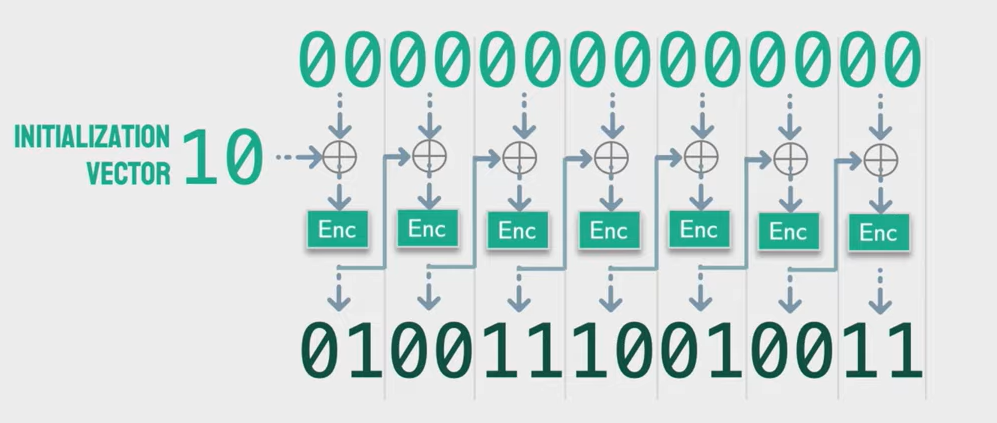
\includegraphics[width=0.6\textwidth]{Photos/Cipher_ Block_Chaining.png}
		\end{SCfigure}
	
		Now another strength of this method is the factor that the same codebook and plaintext can give a wildly different cipher if you just changed the initial seed (or initialisation vector).
		\begin{SCfigure}[0.5][h]
			\caption{This is so nice to look at. Relish the randomness}
			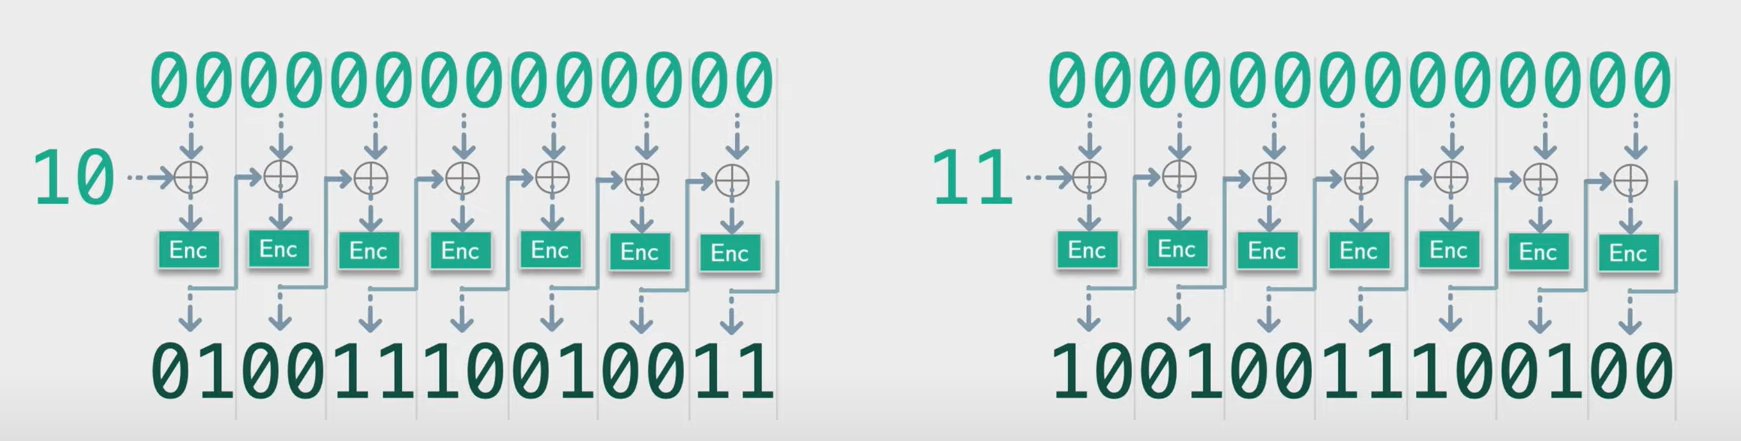
\includegraphics[width=0.6\textwidth]{Photos/CBC_2.png}
		\end{SCfigure}

		\underline{An interesting point}- The I.V. (or initial seed) is not at all a secret. It is in fact given along with the ecrypted message as it is necessary for decryption. Another property - it should not be predictable or used more than once (to ensure resistance from plaintext attacks)

		\subsubsection{How to decrypt CBC}
			\begin{SCfigure}[0.5][h]
				\caption{Decryption exploits the reversibility of \(\oplus\)}
				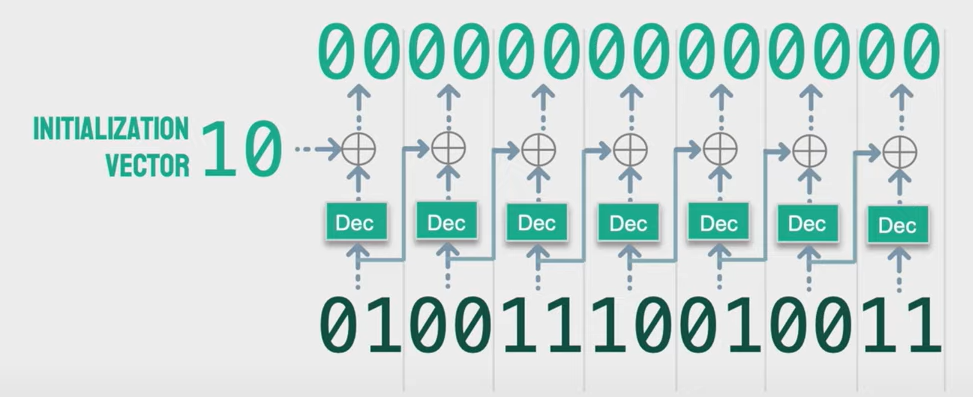
\includegraphics[width=0.6\textwidth]{Photos/CBC_3.png}
			\end{SCfigure}

	\section{Counter Mode (CTR)}
		Another method of Block Ciphering is Counter Mode wherein you are actually encrypting (i.e. using the codebook) on the counter and not the plaintext. The plain text is merely xor-ed with the encryption of the counter. Initial seed decides the starting value of the counter which is incremented.
		\begin{SCfigure}[0.5][h]
			\caption{A very logical and simple encryption process. The counter is on the top and the plaintext is xor-ed in the middle}
			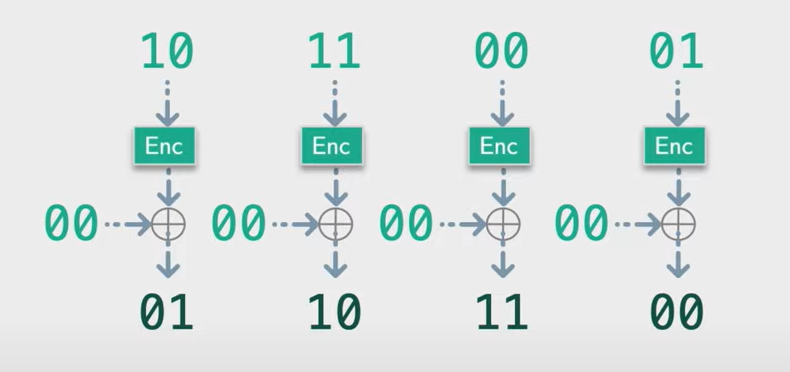
\includegraphics[width=0.6\textwidth]{Photos/CBC_4.png}
		\end{SCfigure}
		
		To put it algebraically, if we called the $k$-bit counter \(C(i)\), and the code book as \(ECB: \{0,1\}^{k} \rightarrow\{0,1\}^k\) and the \(i\)th $k$-bit chunk of plaintext as \(m_i\) then- 
		\begin{mybox}
		\[cipher_i=m_i \oplus ECB(C(i))\]
		\end{mybox}

		\subsection{Decryption}
			\begin{SCfigure}[0.5][h]
				\caption{It is very similar in the sense that we interchange one }
				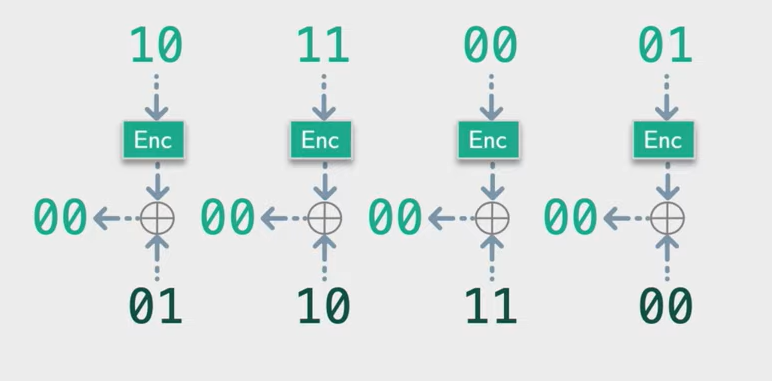
\includegraphics[width=0.6\textwidth]{Photos/CBC_6.png}
			\end{SCfigure}
			In algebraic terms, we can call it- 
			\begin{mybox}
				\[m_i= cipher_i \oplus ECB(C(i))\]
			\end{mybox}

			\begin{center}
			\begin{tabular}{c | c}
				 \hline
				 Advantages over CBC&Disadvantage over CBC\\ 
				 \hline
				 Simpler implementation & Not safe for small block lengths (\(<\)128 bit)\\
				 Resistant to attacks terms as ``padding oracle''& \\
				 \hline  
			\end{tabular}
			\end{center}


